\chapter{Conclusions}\label{C:Conclusions}

This research investigated why programmers do what they do, specifically the influences on their security practices. This chapter will cover conclusions, implications to practice and limitations and future work. Following a Grounded Theory research process, we develop the "Theory of Influences on Security Practices".
\newline
\par
\begin{figure}[ht]
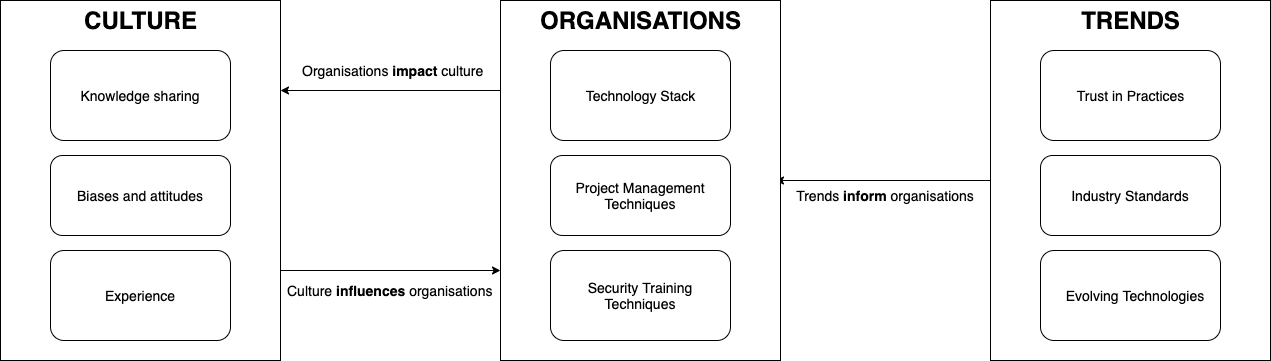
\includegraphics[width=17cm]{figures/fig2.png}
\centering
\caption{The Theory of Influences on Security Practices}
\centering
\end{figure}

\par
Culture referenced knowledge sharing, biases and attitudes. The category is a combination of the culture we see in groups of individuals, and the term culture refers to the customs that programmers have in order to maintain security. Knowledge sharing was internal team communications between members. Biases and attitudes were existing thoughts and feelings on how they implement and learn about security. Experience was the number of the number of threats programmers had been exposed to. 
\newline
\par
Organisations included the attributes, technology stack, project management techniques and security training techniques. The technology stack was the programming languages, libraries, frameworks and tools that were in use by the participants. Project management techniques were management structures enforced within the organisation; whether this is Waterfall, Agile or DevOps. The security training techniques were the avenues of educational support provided by different organisations.  
\newline
\par
Trends specified that trust in practices, industry standards and evolving technologies were due to the influences of industry trends on a programmer. Trust in practices was the lack of checking open-source technology; the industry standard was changing policies, compliance and best-practice standards. Evolving technologies referenced the ever-changing adoption of new technology to business streams.
\newline
\par 
The emergent theory has been evaluated Glaser's criteria of fit, work, relevance and modifiability. It provides a theory which is thoroughly explained, has drawn codes from newly gathered information, is relevant to the topic and can adapt long-term. The theory has also been evaluated against three works of literature. Overall, the findings of this research can provide a more robust educational programme in the workplace and allow for companies to reevaluate how they respond to trends, how they structure their organisations and what they do to improve their culture.

\section{Implications for Practice}

The emergent theory defined three main categories and a further nine attributes for the influences on security practices. By understanding how they each relate to each other, organisations can implement changes in how they react to trends and how they deal with and motivate changes in culture. 
\newline
\par
In New Zealand, there have been some small changes with a participant \textit{[P7] } having completed a Hackathon when joining the organisation, but this change needs to be long-lasting, and there should be constant practical ways to learn about secure programming much like the once a month opportunities that \textit{[P14]} has. This will reinforce security a part of the culture of programmers way-of-working. 
 \newline
 \par
 There needs to be reform in how security is taught in organisations. There should be more support for programmers in terms of technical education within organisations instead of just the general policy and practices that all employees get. Technical education will be best done with frequent, optional internal Hackathons. \textit{[P14]}, described giving cases related to the nature of the organisations work, and this provided a mock scenario which can build up the experiences of employees in a safe environment without any consequences. It also introduces programmers to a diverse technology-stack, and as organisations continue to adapt to the popular trends in the industry, employees need to experience more languages, tools, frameworks, libraries. The range and growth of the experiences which are provided by the organisation in-turn increase the ability for employees to deal with security issues and become more open to changes in the normal day-to-day.  
 \newline
 \par
 Employees will benefit if cross-functional teams are used within organisations. When this trend rises to include security-focused team-members, it will make implementing security in software easier for programmers. Security is a growing field so as the current issues with a lack of money and skillset will reduce as it starts to hold more gain \cite{grow}. 
 

\section{Limitations and Future Work} 

\par There were some limitations in regard to the data collection. While not significant, there was a gender imbalance in the participants. One third were female while the rest male. As women are underrepresented in STEM (Science, Technology, Engineering and Mathematics) fields \cite{wit}, it can be argued that this is indicative of the actual population. However, as women in this industry typically have different experiences to the majority, it would have been interesting to have more varying data to draw codes from \cite{wit}. 
\newline
\par
Another difficulty that limited the theory when data collecting was the refusal to answer questions. Due to non-disclosure agreements, for some participants, this was so strict that they could not answer questions such as, "what language do you use to program with at work?". This made it challenging to draw appropriate conclusions during the middle of this study. This could have also introduced slight biases in the collection as observational inferences were made based on the non-responses. 
\newline
\par
While it was interesting to obtain a diverse range of experiences within the sample group of participants, for future work, the investigation would benefit from reducing this scope. By choosing one type of role, one sector or similar years of experience, the theory would have had some more pointers to technical influences. This would have resulted in critical traits for a programmer to improve upon in their security education directly. It could also provide more insights as to why specific programmers seem to find security a hindrance and how to change this. A suggestion would be to focus on cloud engineers as they were the only ones in this study that indicated that languages and libraries change based on security needs. If future studies could focus on organisational differences, it would be interesting as smaller companies had laxer security controls and support when programming compared to the more prominent companies. Smaller organisations, however, seemed to be more willing and open to change than those in an established organisation.
\newline
\par 
A separate study on internal Hackathons could be undertaken. As it is a relatively new concept in New Zealand and there generally is a paucity of research worldwide, so it would be interesting to combine the two; Corporate Hackathons in New Zealand. Specifically focusing on the differences between less experienced people and more experienced people in terms of work experience and the impacts before, during and after a Hackathon using the Phenomenology methodology could form a strong understanding of the effects on a varying group's experiences due to such an event. It can be used to market the idea of having regular internal Hackathons within organisations in New Zealand. 


